\documentclass[border=3pt]{standalone}
% Shared preamble for every generated figure.
% Matches the report: newtx (Times), greyscale, square boxes.
\usepackage{newtxtext,newtxmath}
% newtx's typewriter (txtt) draws a slashed zero; use Latin Modern instead.
\renewcommand{\ttdefault}{lmtt}
\usepackage{tikz}
\usetikzlibrary{positioning,arrows.meta,calc,fit,backgrounds,shapes.geometric,
                decorations.pathreplacing,decorations.pathmorphing,matrix,patterns}

\definecolor{figgrey}{gray}{0.88}
\definecolor{figmid}{gray}{0.60}
\definecolor{figdark}{gray}{0.35}

\tikzset{
  fig/.style={font=\small},
  box/.style={draw,thick,minimum height=8mm,minimum width=22mm,align=center,
              inner sep=2pt,font=\small},
  greybox/.style={box,fill=figgrey},
  smallbox/.style={draw,minimum height=6mm,minimum width=16mm,align=center,
                   inner sep=2pt,font=\scriptsize},
  ln/.style={-{Stealth[length=2.2mm,width=1.8mm]},thick},
  lnb/.style={{Stealth[length=2.2mm,width=1.8mm]}-{Stealth[length=2.2mm,width=1.8mm]},thick},
  lbl/.style={font=\scriptsize,inner sep=1.5pt},
  note/.style={font=\scriptsize\itshape,inner sep=1.5pt},
}

\begin{document}
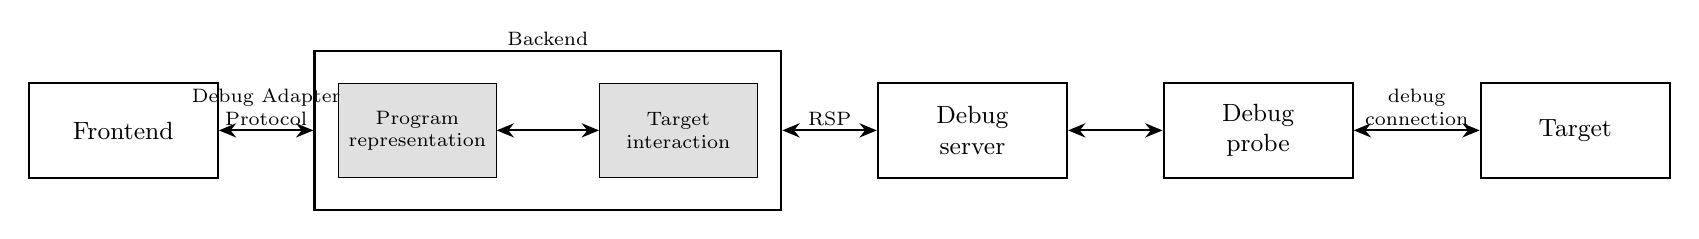
\begin{tikzpicture}[fig]

% --- backend, drawn first so the outer box can be fitted to its contents
\node[smallbox,fill=figgrey,minimum width=20mm,minimum height=12mm] (rep)
      {Program\\representation};
\node[smallbox,fill=figgrey,minimum width=20mm,minimum height=12mm,
      right=13mm of rep] (int) {Target\\interaction};
\draw[lnb] (rep) -- (int);

\begin{scope}[on background layer]
  \node[box,fit=(rep)(int),inner xsep=3mm,inner ysep=4mm] (be) {};
\end{scope}
\node[lbl,anchor=south] at (be.north) {Backend};

% --- the rest of the chain ----------------------------------------------
\node[box,minimum width=24mm,minimum height=12mm,left=12mm of be]  (fe) {Frontend};
\node[box,minimum width=24mm,minimum height=12mm,right=12mm of be] (sv) {Debug\\server};
\node[box,minimum width=24mm,minimum height=12mm,right=12mm of sv] (pr) {Debug\\probe};
\node[box,minimum width=24mm,minimum height=12mm,right=16mm of pr] (tg) {Target};

\draw[lnb] (fe) -- node[lbl,above,align=center]{Debug Adapter\\Protocol} (be);
\draw[lnb] (be) -- node[lbl,above]{RSP} (sv);
\draw[lnb] (sv) -- (pr);
\draw[lnb] (pr) -- node[lbl,above,align=center]{debug\\connection} (tg);

\end{tikzpicture}
\end{document}
